\section{Experimental Setup}
As our projected solution involved a low-cost navigation system, the hardware selection criteria were primarily founded on availability and cost. The cost reduction normally concedes in accurateness and reliability, although with the recent surge of inexpensive, widely accessible, and precise microelectromechanical systems (MEMS), that is no longer the case. Still, we aim to employ commercially available tools at the lowest possible cost without compromising the design of a robust and accurate inertial navigation system. A LoPy microcontroller was selected as the navigational computing device of the inertial system, meeting the envisioned requirements for low power with flexible and diverse computational capabilities. The LoPy development board interfaces with the external physical inertial sensor through connection pins (figure \ref{fig:hardware}.a) and communicates remotely by LoRa protocol. A PySense expansion board connects with the LoPy module providing a programable interface for the microcontroller. The inertial navigation system encompasses a small MPU-9250 (figure \ref{fig:hardware}.b)

\begin{figure}[!h]
    \centering
    \begin{subfigure}{0.45\textwidth}
        \centering
        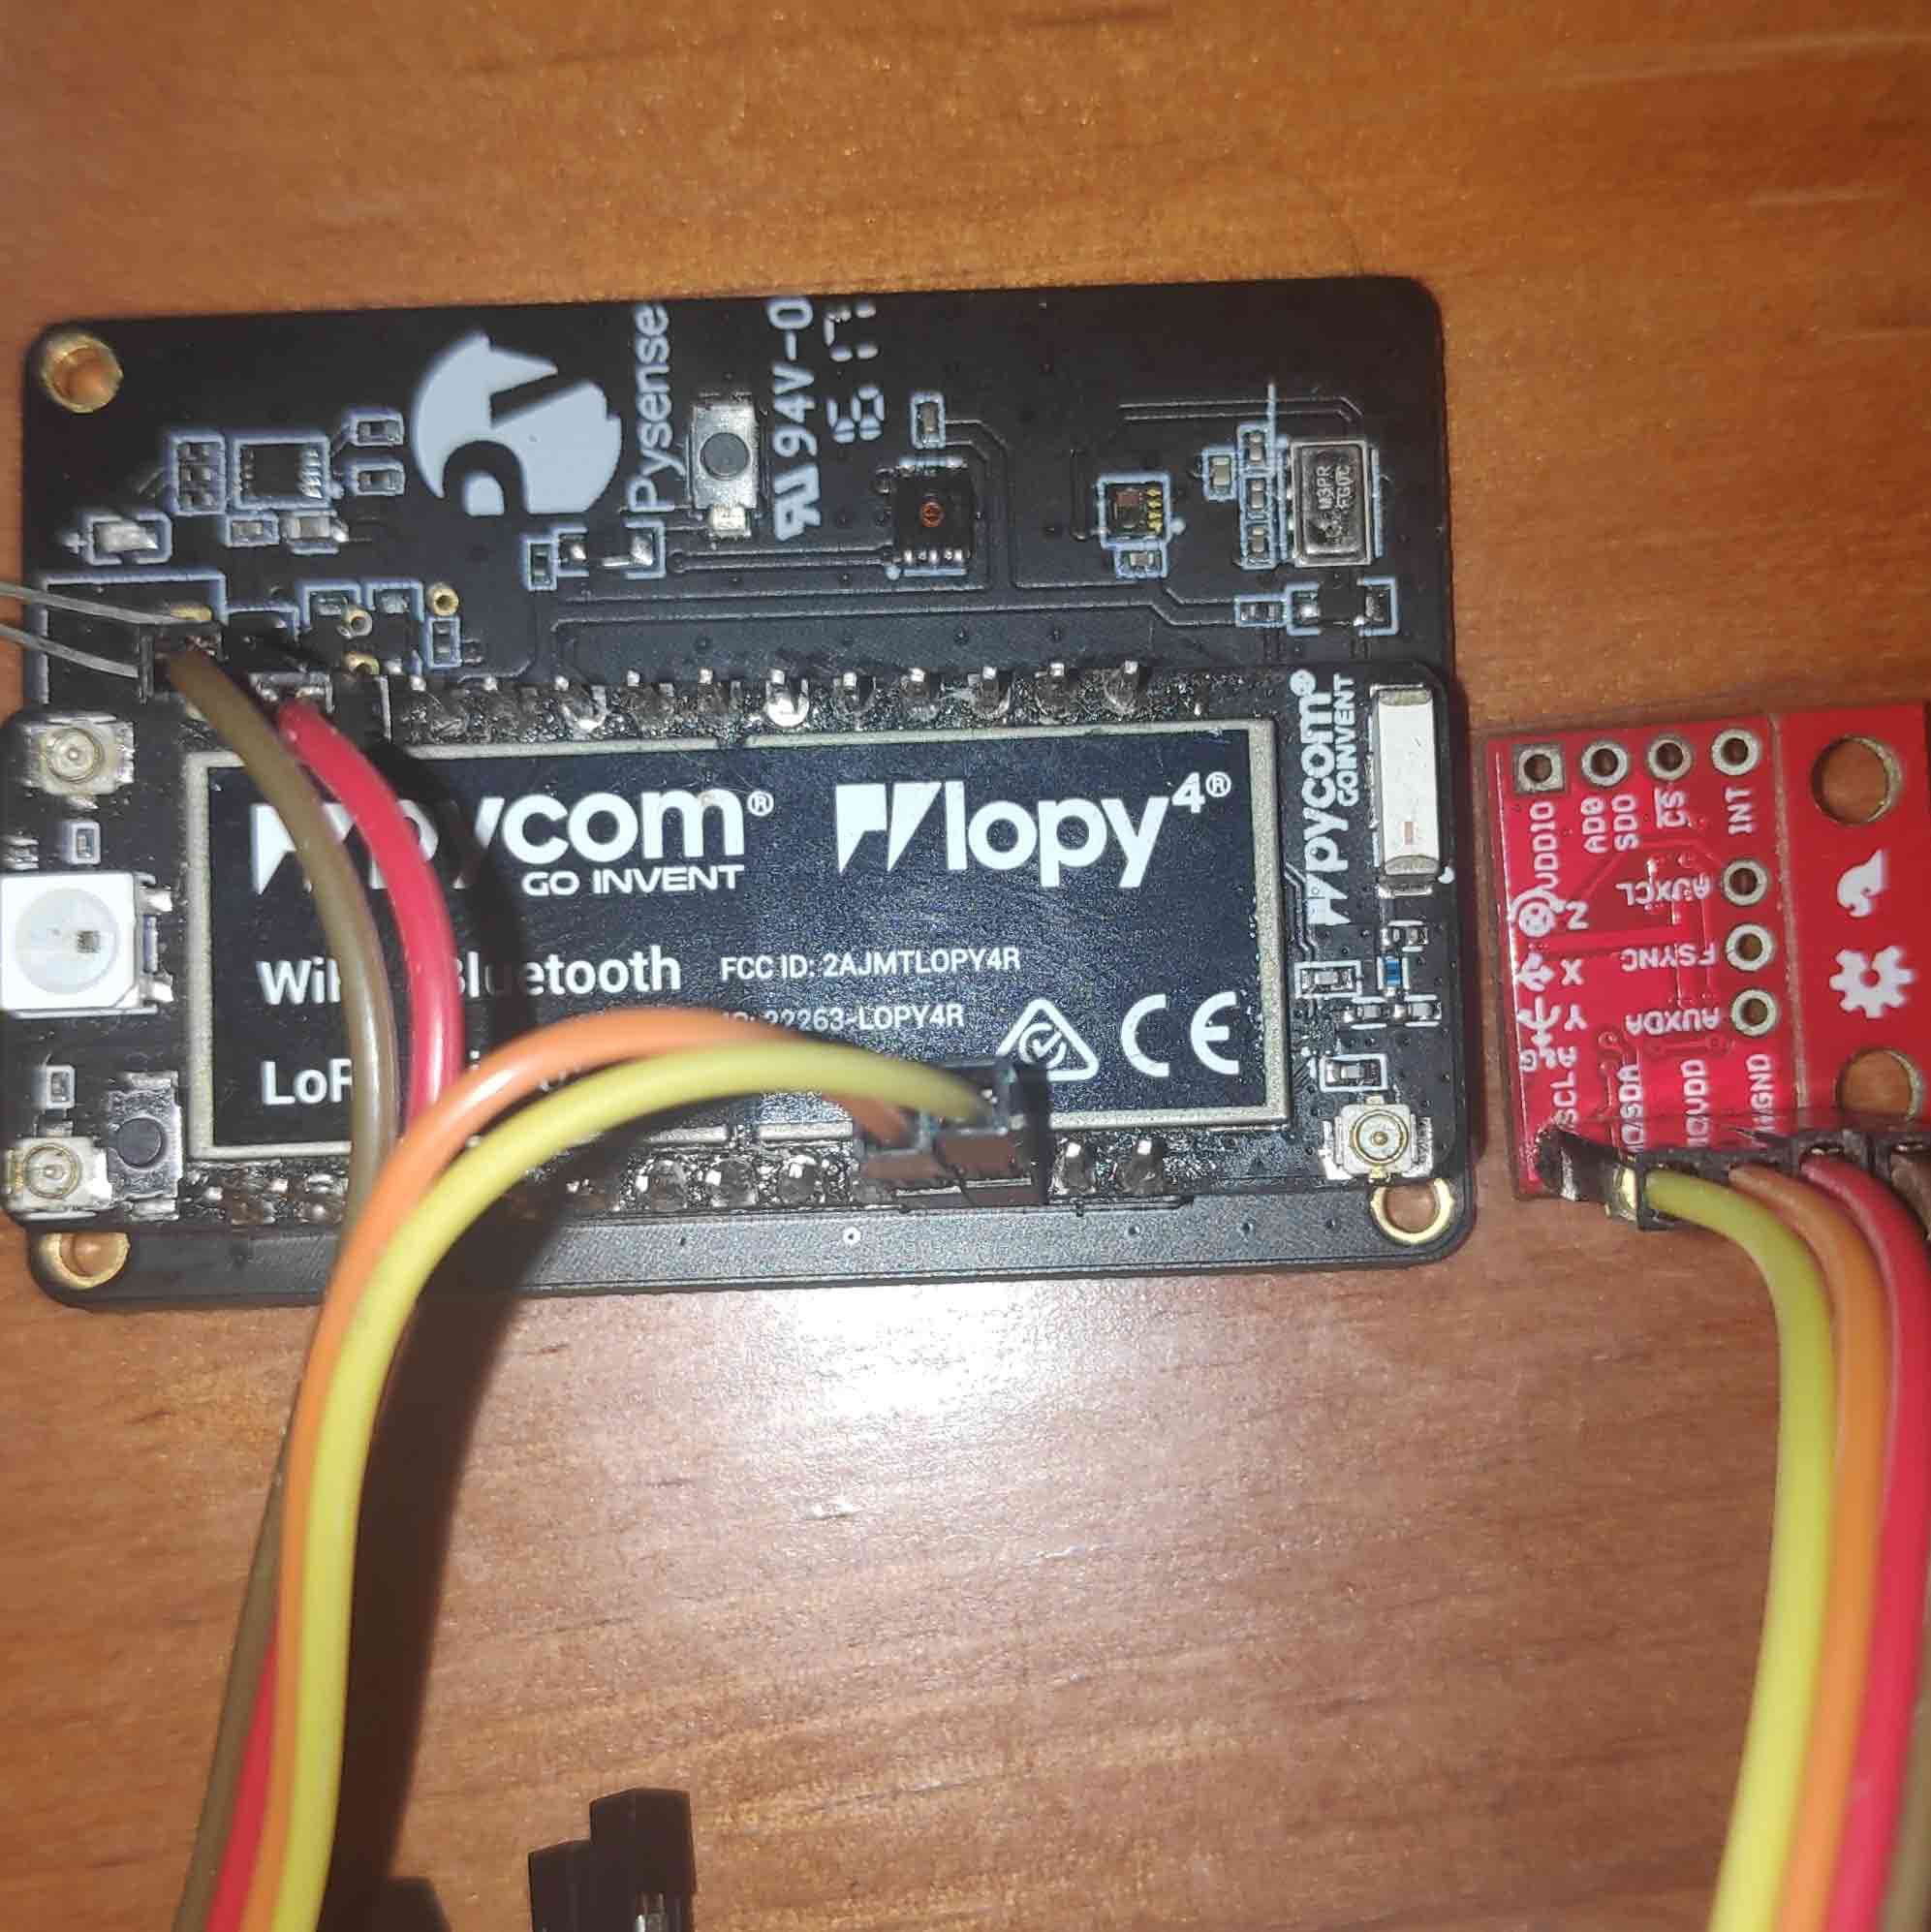
\includegraphics[width=1\textwidth]{figures/INS.jpg}
        \caption{INS Hardware}
        \label{fig:sub1}
    \end{subfigure}%
    \begin{subfigure}{0.45\textwidth}
        \centering
        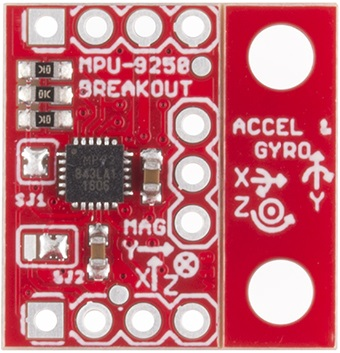
\includegraphics[width=1\textwidth]{figures/mpu9250.jpg}
        \caption{MPU-9250 Breakout}
        \label{fig:sub2}
    \end{subfigure}
    \caption{Pin connection between the microcontroller (left) and the IMU (right). Modules are linked through SCL, CLK, VDD and GND pins.}
    \label{fig:hardware}
\end{figure}

IMU (3x3x1mm) with nine degrees of freedom comprising three accelerometers, three orthogonal gyros, three magnetometers as well as temperature and pressure sensors. This chip is extensively employed in wearable sensors for health, fitness, and sports, motion-based game controllers, and portable gaming. A correct calibration of such sensors is essential for the compensation of their systematic errors, bias, and scale factor. Each time prior to an experiment, the inertial sensor is calibrated while the system is stationary and stabilized to compensate for static error that might corrupt the measurements.
\begin{table}[H]
    \begin{center}
        \begin{tabular}[t]{lcccc}
            \hline
            Parameter                   & Min. & Typ.      & Max.   & Units             \\
            \hline
            Full-Scale range            &      & $\pm 16$  &        & $g$               \\
            Sensitivity Scale Factor    &      & 2,048     &        & $LSB/g$           \\
            Nonlinearity                &      & $\pm 0.1$ &        & $\%$              \\
            Rate Noise Spectral Density &      & 300       &        & $\mu g/\sqrt{Hz}$ \\
            Operating Current           &      & 3.2       &        & $mA$              \\
            Startup Time                &      & 20        &        & $ms$              \\
            Output Data Rate            & $4$  &           & $4000$ & $Hz$              \\
            \hline
        \end{tabular}
        \caption{Accelerometer Specifications. }
        \label{tab:accelerometer_specification}
    \end{center}
\end{table}

\begin{table}[H]
    \begin{center}
        \begin{tabular}[t]{lcccc}
            \hline
            Parameter                   & Min. & Typ.       & Max.   & Units                  \\
            \hline
            Full-Scale range            &      & $\pm 2000$ &        & $^{\circ}/s$           \\
            Sensitivity Scale Factor    &      & 131        &        & $LSB/(^{\circ}/s)$     \\
            Nonlinearity                &      & $\pm 0.5$  &        & $\%$                   \\
            Rate Noise Spectral Density &      & 300        &        & $^{\circ}/s/\sqrt{Hz}$ \\
            Operating Current           &      & 450        &        & $\mu A$                \\
            Startup Time                &      & 35         &        & $ms$                   \\
            Output Data Rate            & $4$  &            & $8000$ & $Hz$                   \\
            \hline
        \end{tabular}
        \caption{Gyroscope Specifications. }
        \label{tab:gyroscope_specification}
    \end{center}
\end{table}

\begin{table}[H]
    \begin{center}
        \begin{tabular}[t]{lcccc}
            \hline
            Parameter                     & Min. & Typ.       & Max. & Units        \\
            \hline
            Full-Scale range              &      & $\pm 4800$ &      & $\mu T$      \\
            Sensitivity Scale Factor      &      & 0.6        &      & $\mu T/ LSB$ \\
            Operating Current             &      & 280        &      & $\mu A$      \\
            Initial Calibration Tolerance &      & $\pm 500$  &      & $LSB$        \\
            \hline
        \end{tabular}
        \caption{Magnetometer specification. }
        \label{tab:magnetometer_multiplication}
    \end{center}
\end{table}

The microcontroller operates MicroPython, a barebones and efficient implementation of Python 3, which incorporates a small subset of the Python standard library. It is optimized to run on microcontrollers and in constrained environments. The inertial module's raw measurements are interpreted by the microcontroller through Inter-Integrated Circuit (I2C) MicroPython driver serial allowing to read the peripherals memory addresses synchronously. The readings of each sensor are later averaged and linearized to better detect and reduce the presence of outlier readings. A fusion algorithm takes as input the averaged data of the accelerometer, gyroscope, and magnetometer. It returns the estimated inertial angles (pitch, roll, and yaw) as well as the projected linear acceleration with a gravity compensation numerical method that utterly removes the effect of the gravity component. Numerically integrating the resultant linear acceleration yields velocity, and double integrating will deliver the body's accumulative position. Merging the AHRS with an accumulative position allows tracking a moving body in three dimensions over time. Moreover, the navigation system is equipped with a LoRa antenna enabling the system to transmit at 868MHz/915MHz LoRa bands in real-time at a long distance the position and orientation information to an external gateway (figure \ref{fig:overview}). A visualization of the entire hardware solution is provided at image \ref{fig:full}.

\begin{figure}[!h]
    \centering
    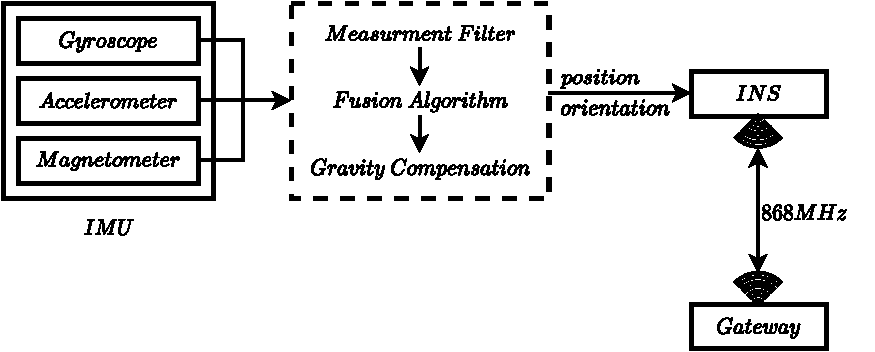
\includegraphics[width=0.9\textwidth]{figures/overview.pdf}
    \caption{System overview - Raw measurements from IMU are fused together and numerically integrated to obtain position and orientation. This INS data is transmitted in real-time to a remote node gateway. }
    \label{fig:overview}
\end{figure}

\begin{figure}[!h]
    \centering
    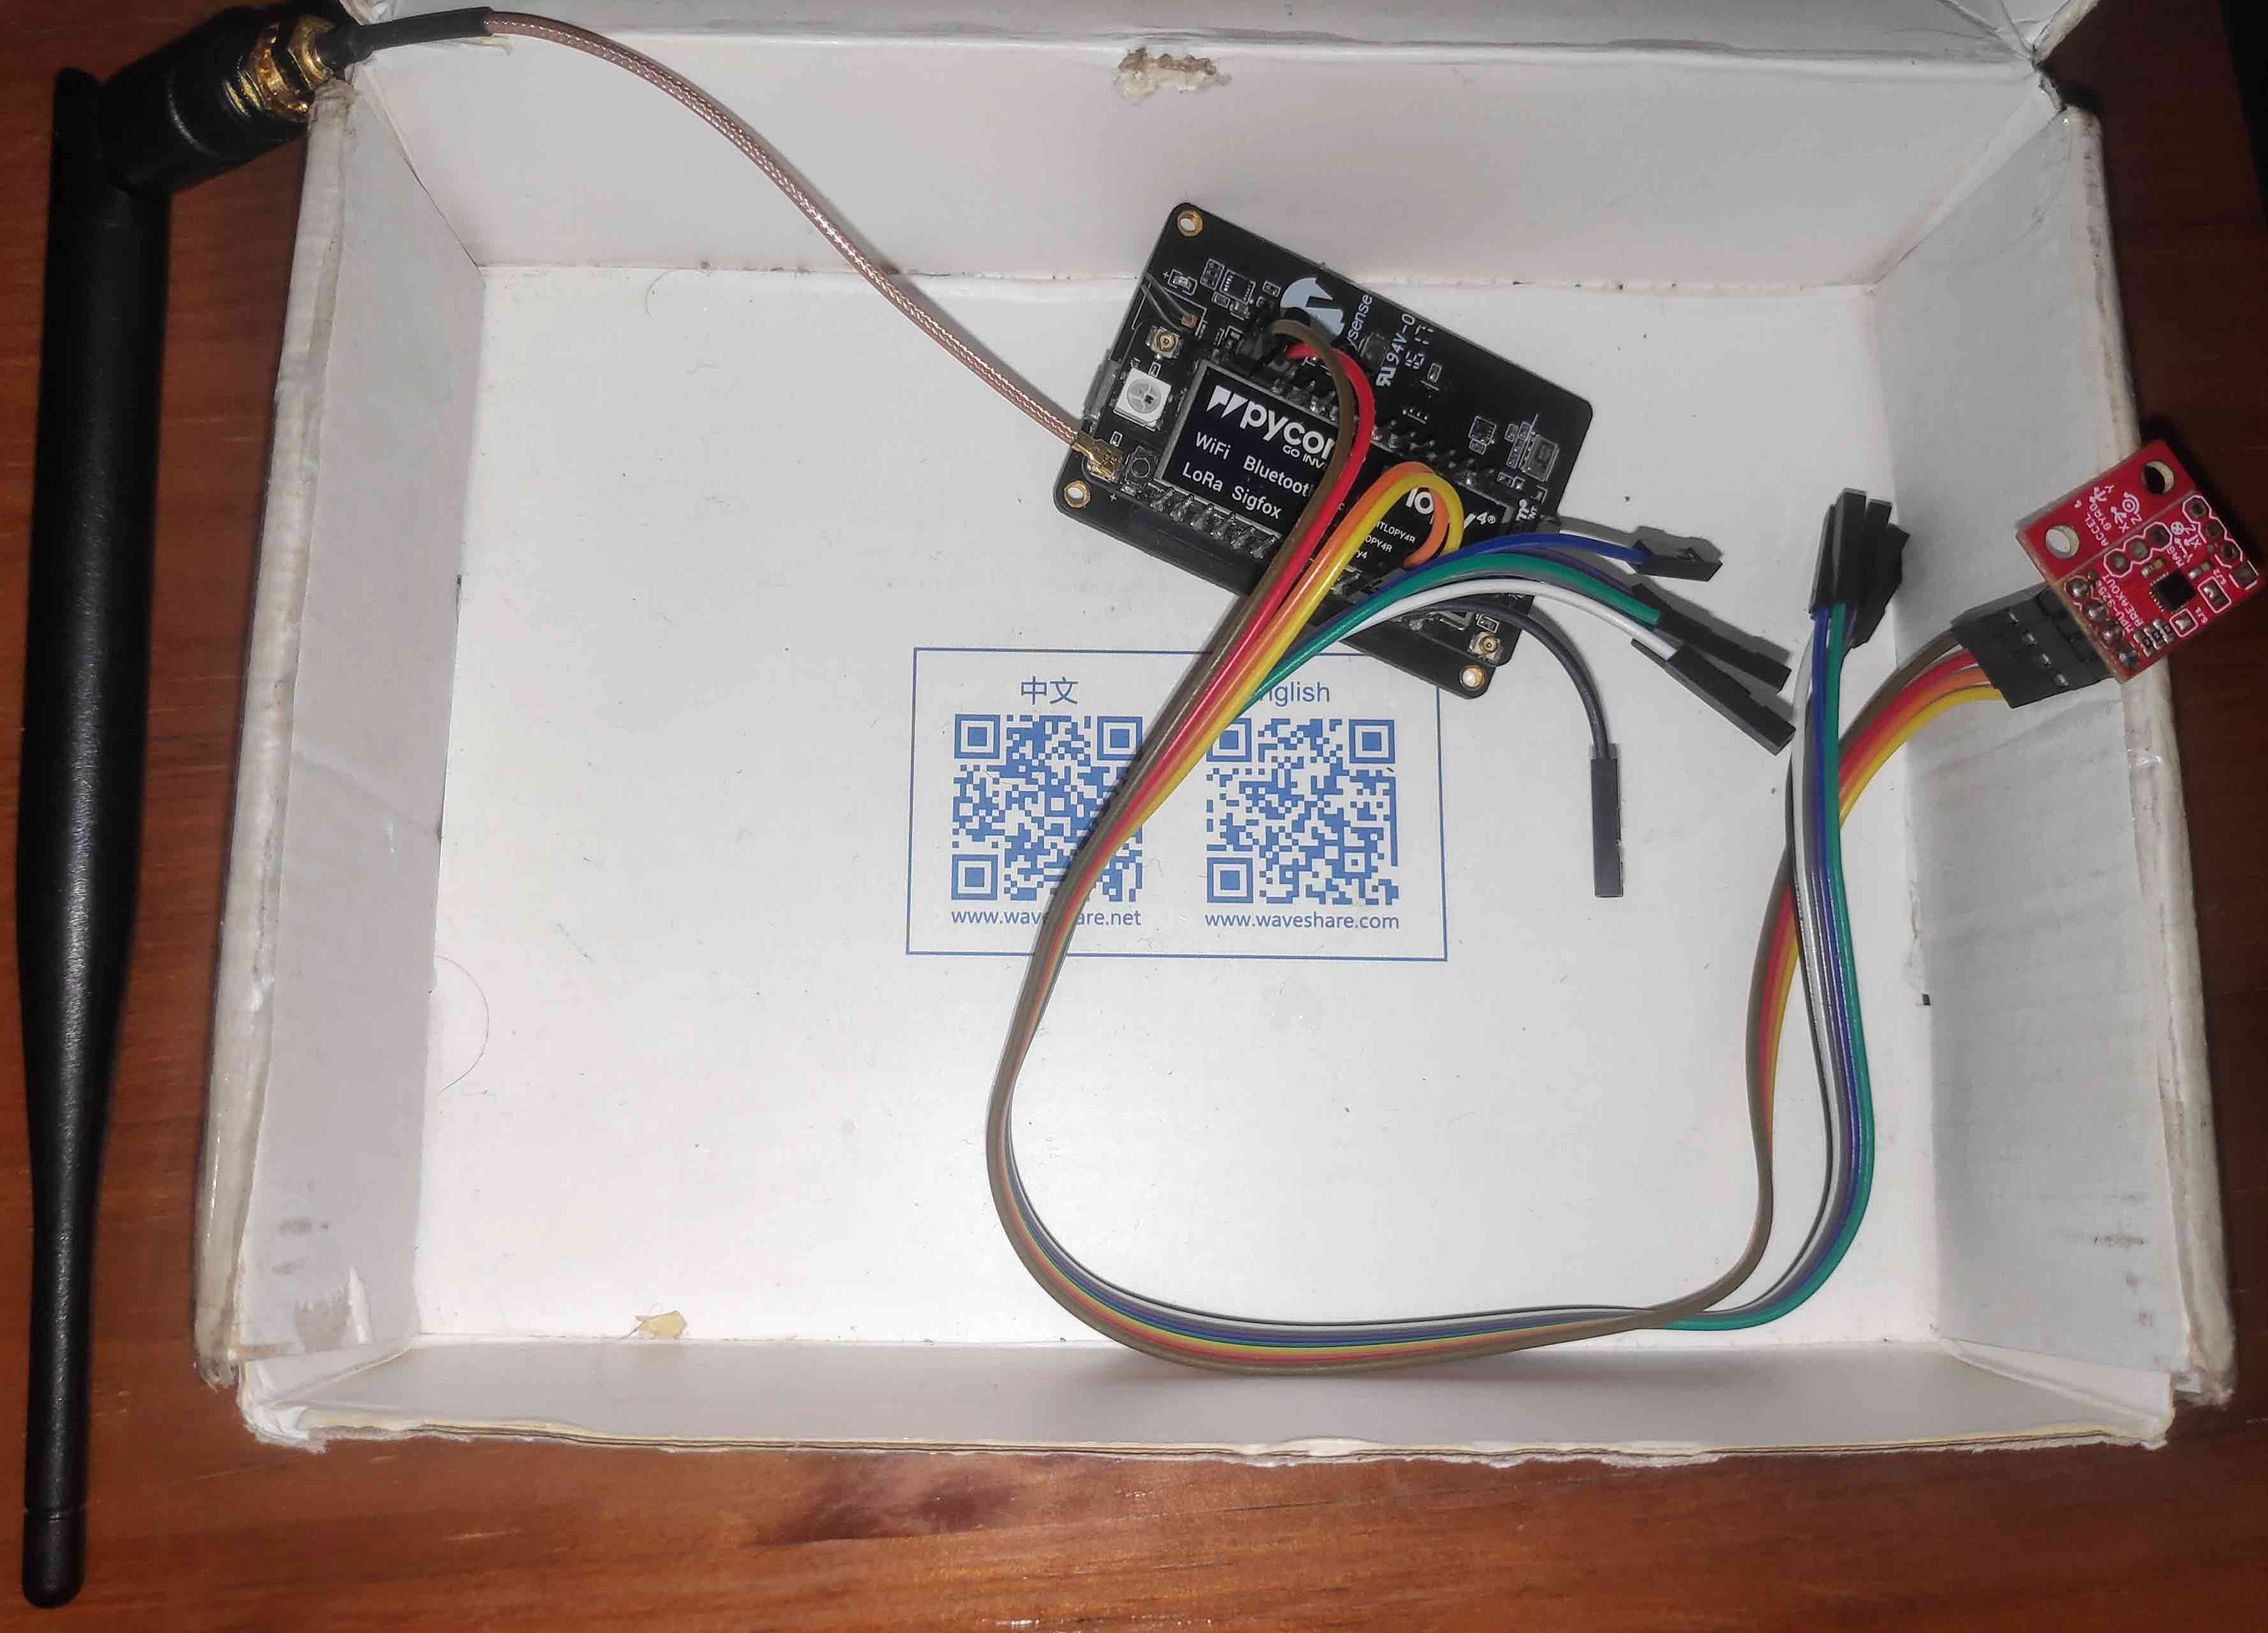
\includegraphics[width=0.9\textwidth]{figures/fullINS.jpg}
    \caption{Complete hardware solution - Box containing the full inertial navigation system, at the left the antenna  suitable for use in the 868MHz/915MHz LoRa bands. }
    \label{fig:full}
\end{figure}
\subsection{Indoor Experiments}
\begin{figure}[!h]
    \centering
    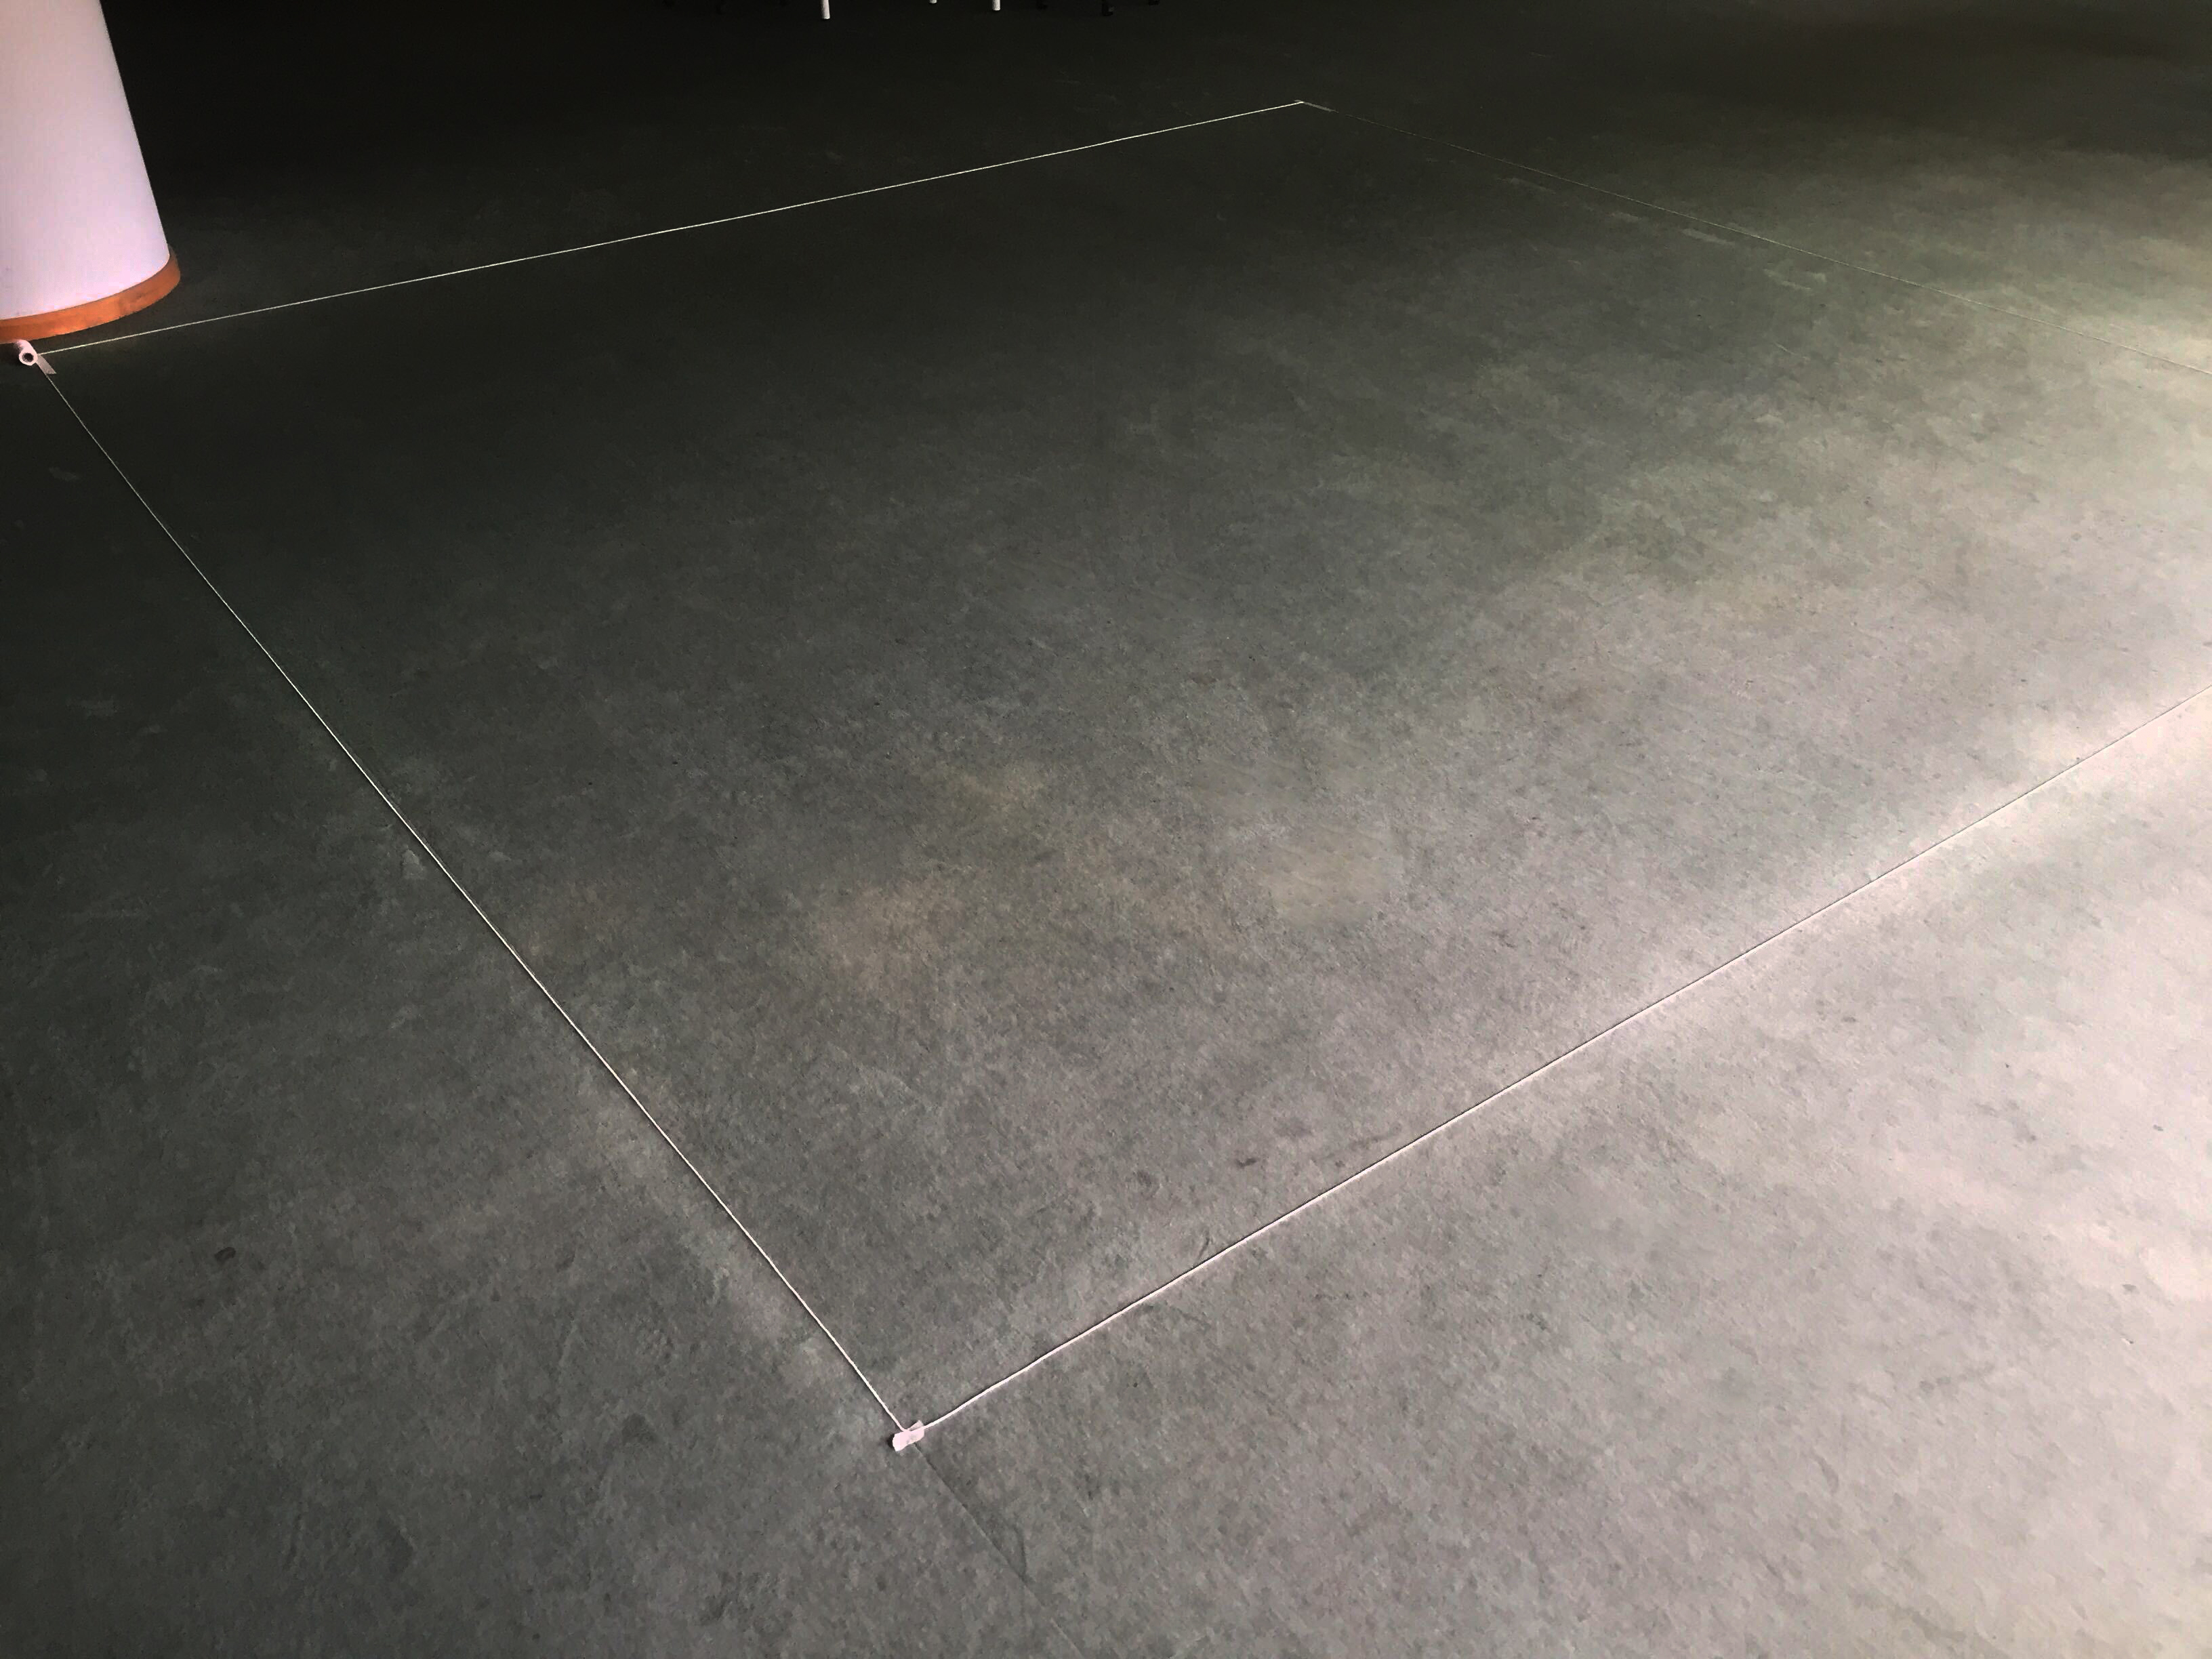
\includegraphics[width=0.9\textwidth]{figures/indoor.jpg}
    \caption{ 5 meter side ground square used for baseline of accuracy of inertial system. }
    \label{fig:indoor}
\end{figure}

\begin{figure}[!h]
    \centering
    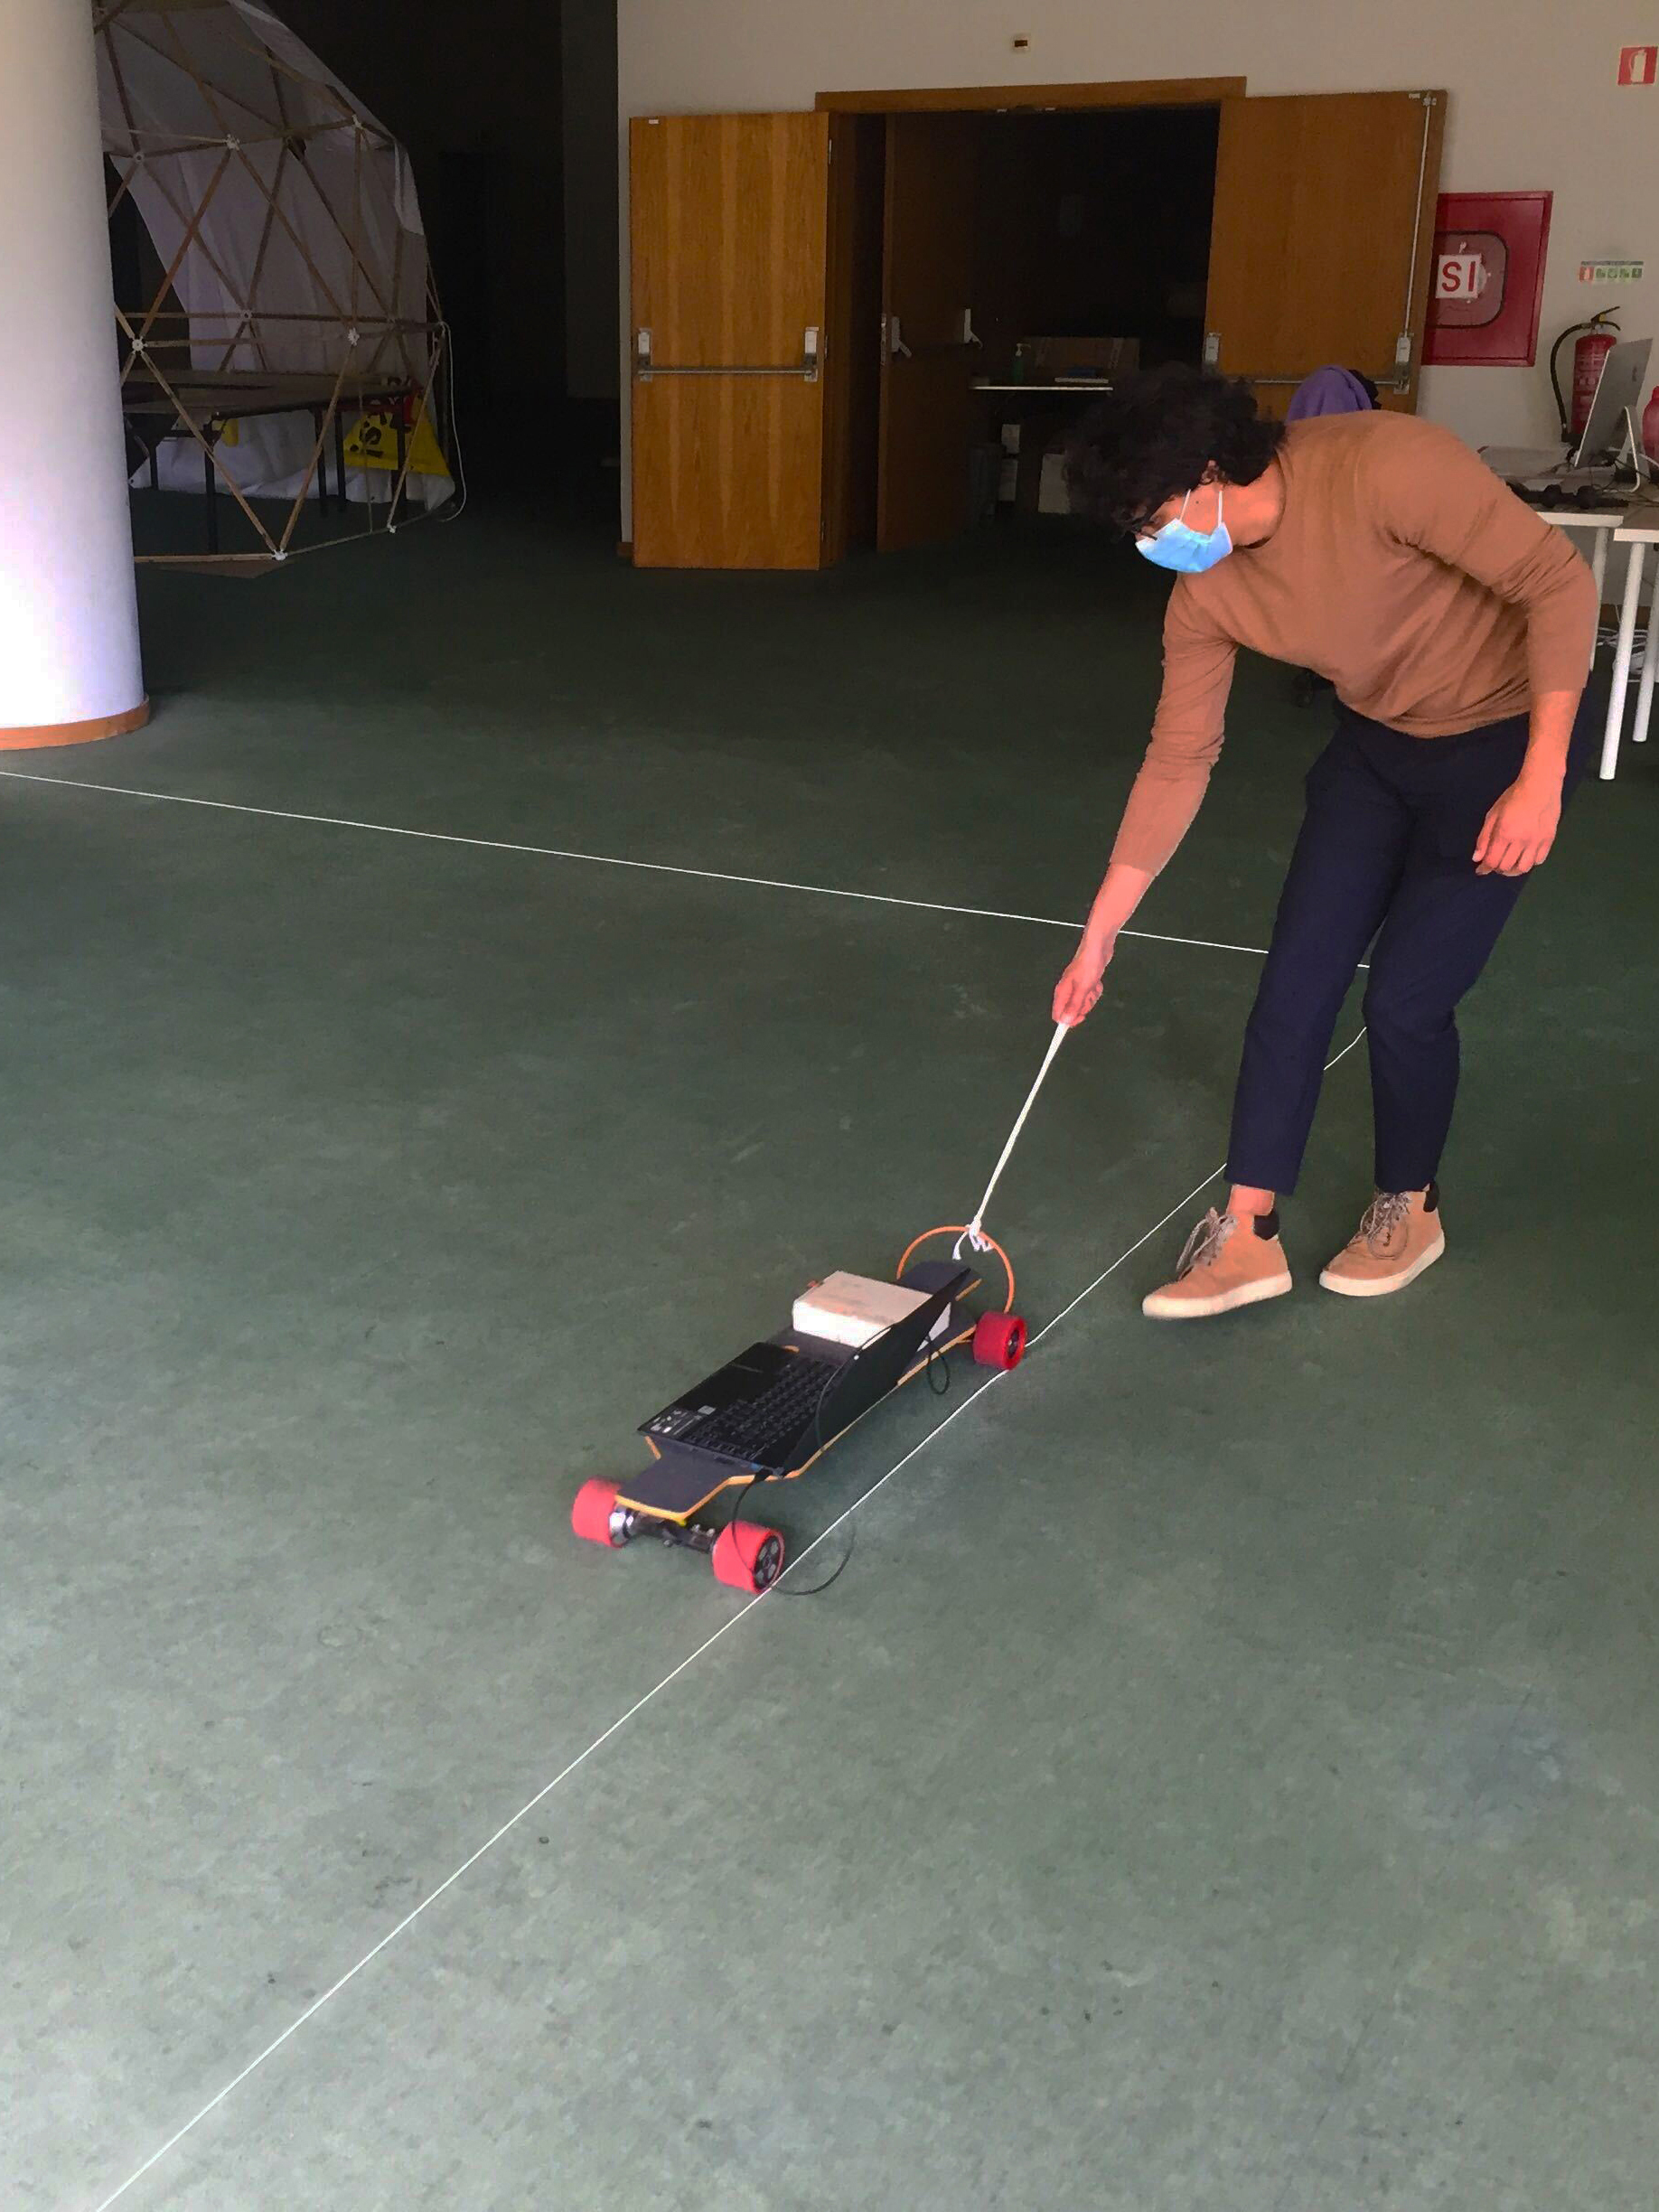
\includegraphics[width=0.9\textwidth]{figures/indoor_1.jpg}
    \caption{ Manually pulling the skateboard on each side of the ground square. }
    \label{fig:indoor_1}
\end{figure}

\begin{figure}[!h]
    \centering
    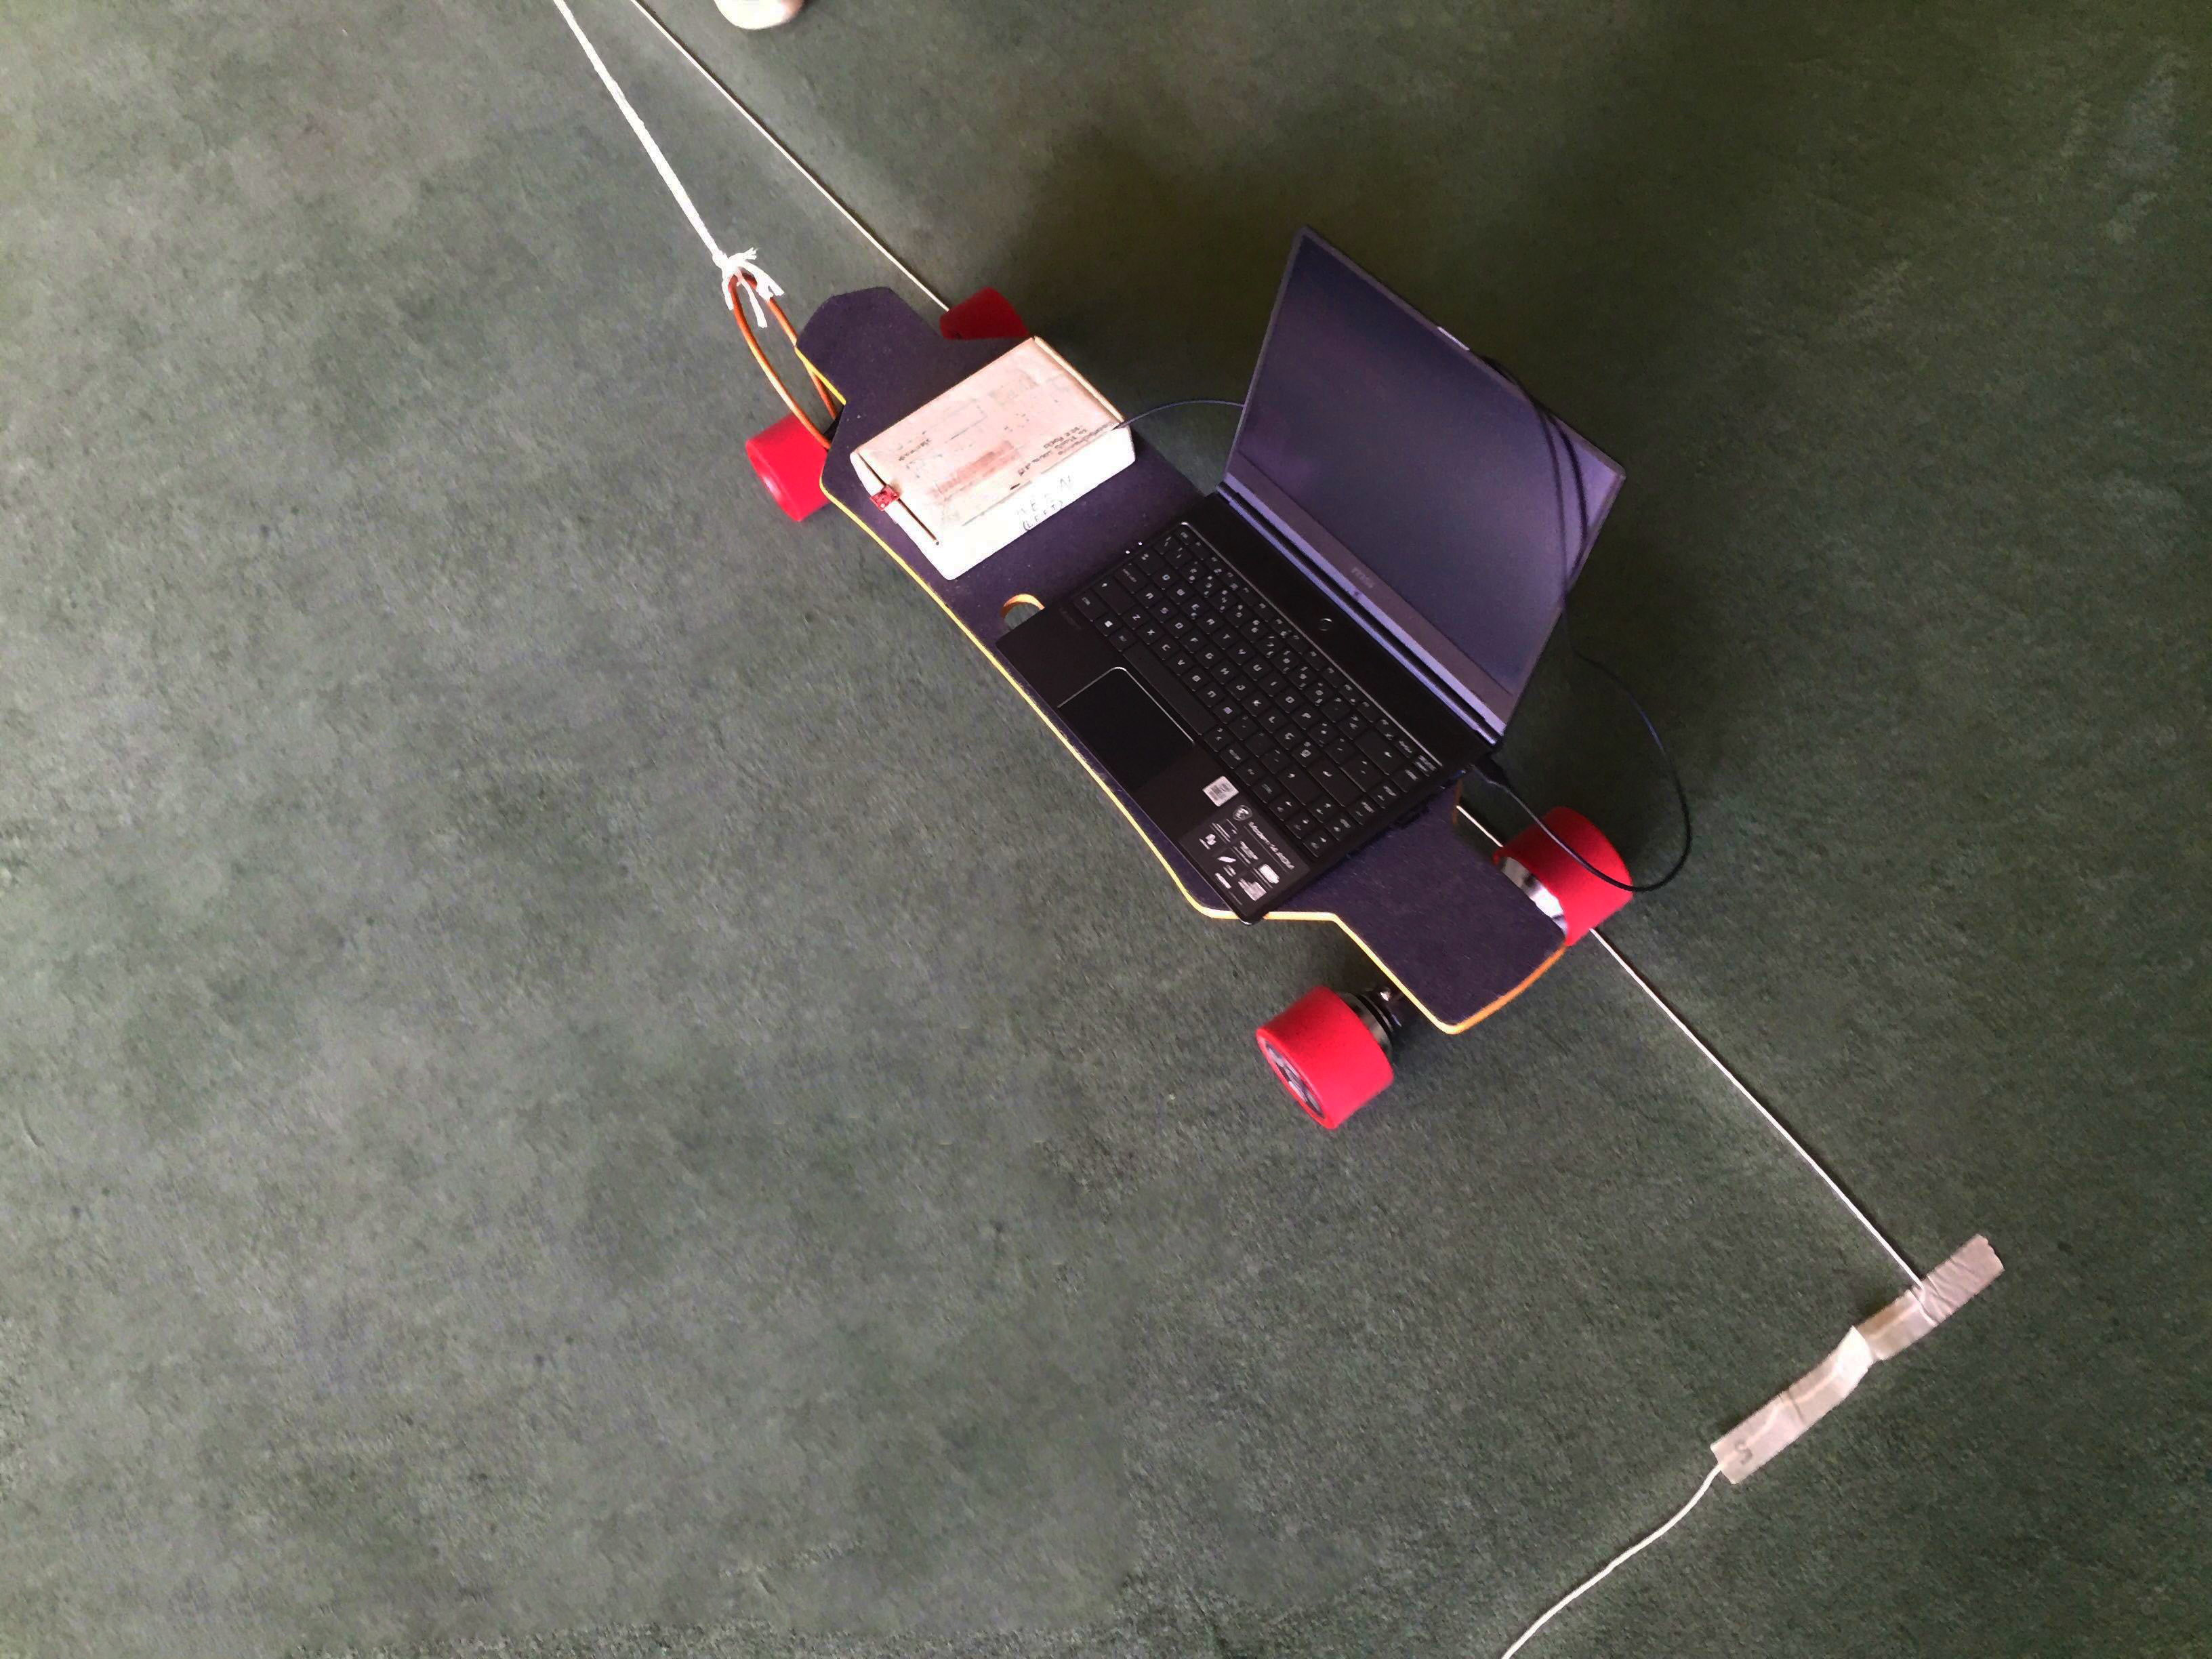
\includegraphics[width=0.9\textwidth]{figures/indoor_2.jpg}
    \caption{ Experiment made with skateboard to assess localization accuracy. }
    \label{fig:indoor_2}
\end{figure}

\subsection{Outdoor Experiments}
